\documentclass{report}
\usepackage[utf8]{inputenc}
\usepackage{hyperref}
\usepackage{amsmath}
\usepackage{bera}
\usepackage{listings}
\usepackage{xcolor}
\usepackage{graphicx}

\graphicspath{{../../figures/}}

\title{
    {Moral AI IQP}\\
    {\large Worcester Polytechnic Institute}\\
    {
\includegraphics[height=2in]{figures/WPI_Inst_Prim_FulClr.png}}
}
\author{Ryan Benasutti}
\date{March 2019}

\newcommand{\code}{\texttt}

\begin{document}

\maketitle

\clearpage
\mbox{}
\clearpage

\chapter*{Abstract}

Artificial intelligence is being deployed in increasingly autonomous systems where it will have to
make moral decisions. However, the rapid growth in artificial intelligence is outpacing the
research in building explainable systems. In this paper, a number of problems around one facet of
explainable artificial intelligence, training data, are explored. A solution to these problems is
presented.

\chapter*{Executive Summary}

Background:
\begin{enumerate}
    \item AI will soon have to make moral decisions, so it should be designed to be fair.
    \item In order to verify AI's fairness, testing must be employed.
\end{enumerate}

Research Objectives:
\begin{enumerate}
    \item Determine at what severity of bias in training data the neural network becomes biased.
    \item Show that neural network testing is possible and necessary.
    \item Survey a small audience to determine the thought processes behind making moral decisions.
\end{enumerate}

Research Methodology:
\begin{enumerate}
    \item Use a graphical model to generate training and test data with controlled bias.
    
    \item Develop a neural network and train it on many different biased training data sets using
    supervised learning and evaluate its accuracy to determine where it becomes biased.
\end{enumerate}

Findings and Analysis:
\begin{enumerate}
    \item The neural network became biased when ...
    
    \item This shows that neural network testing is necessary.
    
    \item We recommend that training data sets omit attributes such as ... in order to avoid
    training a biased neural network.
\end{enumerate}

\chapter*{Acknowledgements}

\begin{enumerate}
    \item Professor Therese Smith
    \item Professor Yunus Telliel
    \item Griffin Tabor
\end{enumerate}

\tableofcontents

\chapter{Introduction}

\begin{enumerate}
    \item Autonomous vehicle technology is growing rapidly and AI is a key piece of that technology.
    As this technology gets closer to attaining full autonomy, the AI deployed in these systems will
    have greater responsibility than ever. These AI systems must be explainably fair, i.e. they must
    both make decisions using only the least amount of information necessary for optimal performance
    and make those decisions predictably and correctly. For example, the AI in an autonomous vehicle
    does not need to be supplied with information about a pedestrian's race, even though race may be
    an impactful trait in other fields, especially medical fields \cite{sickeCellDisease}.
    Furthermore, these AI systems must also be explainable for legal reasons, such as determining
    which party is at fault in the event of a car accident or, in the European Union, complying with
    a user's "right to explanation" \cite{goodman2017european}.
    
    \item The demand for explainable AI is increasing, such as DARPA's Explainable Artificial
    Intelligence (XAI) program \cite{gunning2016explainable}. This program aims to develop
    explainable AI systems such as in Figure~\ref{fig:darpa_xai}.
    
    \item There is an audience which wants to learn more about AI and is a good candidate to educate
    about AI testing.
    
    \item We seek to empirically demonstrate how an AI can learn a bias and the severity of that
    bias. Testing can be employed to evaluate the severity of a bias.

    \item We also seek to understand the decision making process in humans behind making moral
    decisions in unavoidable accident scenarios, i.e. dilemmas.
\end{enumerate}

\chapter{Background}

\begin{enumerate}
    \item Introduce background readings.
    
    \item Cite examples of AI that must (or will in the near future) make moral decisions.
    \begin{itemize}
        \item \cite{bojarski2016end} performs end-to-end learning which "map raw pixels from a
        single front-facing camera directly to steering commands". With this approach, the AI will
        have to directly respond to pedestrians and other external stimuli.
    \end{itemize}
    
    \item The Moral Machine experiment \cite{awad2018moral} is prior research into people's
    preferences in moral dilemmas. Participants are shown a moral dilemma involving an autonomous
    vehicle, passengers, and pedestrians. In each dilemma, the participant must choose between
    inaction, which results in the certain death of the pedestrians, and action, which results in
    certain death of the passengers. The study revealed three strong global preferences towards
    sparing humans over animals, sparing more lives rather than fewer, and sparing younger lives
    rather than older. The study also showed that some preferences vary between countries depending
    on that country's propensity towards egalitarianism.
    
    \item Discuss the Rio Inclusive AI conference. This is our target audience.
\end{enumerate}

\chapter{Methods}

\section{Data Generation}

The data is generated using a graphical model to control the conditional probabilities for the
states of each variable. The variables in the model correspond directly to the attributes of a
person. Figure~\ref{fig:graphical_model_image} is a rendering of the graphical model. For example,
people in the first option could be more likely to jaywalk then people in the second option,
producing a data set which is biased towards/against jaywalkers. When combined with control over the
number of people in each option, this method can produce both subtle and strong bias. The code for
the domain of each attribute of a person is in Figure~\ref{fig:code_for_person_attribute_domains}.
\href{https://github.com/pgmpy/pgmpy}{pgmpy} is used to create the graphical model and infer each
variable’s probability distribution. These distributions are then used to pick elements from each
variable’s domain. This process is repeated for each attribute of each person and for the num- ber
of people in each option of a dilemma, forming a complete dilemma. The number of dilemmas generated
is specified programmatically using the \code{TrainMetadata} class, which captures the number of
dilemmas to generate and the maximum number of people per option.

\begin{figure}
    \centering
    \begin{verbatim}
    age_states = [10, 20, 30, 40, 50, 60]
    race_states = [Race.white, Race.black, Race.asian,
                Race.native_american, Race.other_race]
    legal_sex_states = [LegalSex.male, LegalSex.female]
    jaywalking_states = [False, True]
    driving_under_the_influence_states = [False, True]
    \end{verbatim}
    \caption{Python code for the bracketed attributes of a Person}
    \label{fig:code_for_person_attribute_domains}
\end{figure}

\section{Data Bracketing}

Attributes are one-hot encoded so the neural network is resilient to unspecified attributes. Age is
bracketed by increments of 10 years. Some example encoded ages are shown in
Table~\ref{tab:example_age_attribute_encoding}. Boolean attributes are encoded into three
increments, as shown in Table~\ref{tab:example_boolean_attribute_encoding}.
    
\begin{table}
    \centering
    \begin{tabular}{c|c|c|c|c|c|c|c}
        Age (yr) & unspecified & 1-10 & 11-20 & 21-30 & 31-40 & 41-50 & 51-60 \\\hline
        unspecified & 1 & 0 & 0 & 0 & 0 & 0 & 0 \\
        0 & 0 & 1 & 0 & 0 & 0 & 0 & 0 \\
        3 & 0 & 1 & 0 & 0 & 0 & 0 & 0 \\
        16 & 0 & 0 & 1 & 0 & 0 & 0 & 0 \\
        42 & 0 & 0 & 0 & 0 & 0 & 1 & 0
    \end{tabular}
    \caption{Example age attribute encoding.}
    \label{tab:example_age_attribute_encoding}
\end{table}

\begin{table}
    \centering
    \begin{tabular}{c|c|c|c}
        Value & unspecified & false & true \\\hline
        unspecified & 1 & 0 & 0 \\
        false & 0 & 1 & 0 \\
        true & 0 & 0 & 1
    \end{tabular}
    \caption{Example boolean attribute encoding.}
    \label{tab:example_boolean_attribute_encoding}
\end{table}

\section{Data Storage}

Data is stored using the JSON format, which was chosen because it is popular and easily
machine-readable. The purpose of storing the generated data sets is to keep the data consistent
between test iterations and to share the data. JSON is the chosen data format because it is popular
and is easily machine-readable. After generation, the training and test data sets are stored in
JSON-encoded files using \href{https://jsonpickle.github.io/}{jsonpickle}.

\section{Neural Network Model}

The requirements of the neural network used in the experiments are:
\begin{enumerate}
    \item The network must classify the training data. In other words, when given a dilemma, the
    network must classify that dilemma based on which option is most preferable. For example, in a
    dilemma with two options of three and four people, respectively, the correct classification is
    the second option because it has more people. In the case where a dilemma has two or more
    options of equal size, the earlier option is chosen.
    
    \item The network must be easy to train, meaning that the time required to train the network
    must be small (on the order of minutes or less) and the hardware resources required to train the
    network must be minor. Testing the network requires training it many times, so the time required
    to train the network must be small. Additionally, the network will be trained on personal
    machines, so hardware requirements must be easy to meet.
\end{enumerate}

The final neural network chosen is a simple neural network with one hidden layer trained using
supervised learning. The alternative models considered are:
\begin{enumerate}
    \item An autoencoder. Autoencoders are trained using unsupervised learning, so labeling the data
    is not necessary (want to avoid imparting a set of morals). This model would perform
    dimensionality reduction, and perhaps learn to ignore noise (i.e. uniformly distributed
    attributes) in the data set, but would be unable to classify the dilemmas.
    
    \item An autoencoder in combination with a simple neural network trained using supervised
    learning. This model solves the classification problem which the previous model failed at, but
    introduced unnecessary complexity to the research. The intent of this research is not to build a
    neural network capable of guiding a real autonomous vehicle.
    
    \item A recurrent neural network (RNN) with long short-term memory (LSTM). This option was
    considered because RNN's are capable of accepting variable-length sequential data; however, this
    network does not solve the classification problem, so it is unusable for this research.
\end{enumerate}

\section{Neural Network Training}

The neural network is modeled and trained using Keras. The input layer has dimensionality equal to
the number of attributes per person (after one-hot encoding) multiplied by the number of options per
dilemma multiplied by the maximum number of people per option. The output layer has dimensionality
equal to the number of options per dilemma. The hidden layer has dimensionality equal to the average
of that of the input and output layers. An example implementation can be seen in
Figure~\ref{fig:code_for_keras_model}.

\begin{figure}
    \centering
    \begin{verbatim}
    output_dim = 2
    input_dim = 22 * output_dim * \
            train_metadata.max_num_people_per_option

    model.add(Dense(units=input_dim, activation='relu',
                input_dim=input_dim))
    model.add(Dense(units=round((input_dim + output_dim) / 2),
                activation='relu'))
    model.add(Dense(units=output_dim, activation='softmax'))
    \end{verbatim}
    \caption{The Keras code for the neural network model.}
    \label{fig:code_for_keras_model}
\end{figure}

\section{Neural Network Testing}

The neural network is tested using Keras to evaluate the classification accuracy and loss against a
test data set. The test data is generated in the same way as the training data, though typically
with less or no bias. Each training data set is tested five times. Each iteration involves training
the neural network on the training data set and evaluating its performance against a test data set
to collect classification accuracy and loss information. The results of all five runs are averaged
to produce an average classification accuracy and loss.

\chapter{Findings and Analysis}

\begin{enumerate}
    \item Our research found that the AI became biased when ...
    
    \item Our recommendation to avoid biased AI is to format the training data such that ...
    
    \item The survey results were ... and we extrapolate that the thought process behind these moral
    decisions is ...
\end{enumerate}

\chapter{Conclusion}

\begin{enumerate}
    \item Our research found that AI becomes biased when ...
    
    \item In order to avoid biased AI, we recommend formatting training data such that ...
\end{enumerate}

\bibliography{citations}
\bibliographystyle{plain}

\appendix
\chapter{Figures}

\begin{figure}[h]
    \centering
    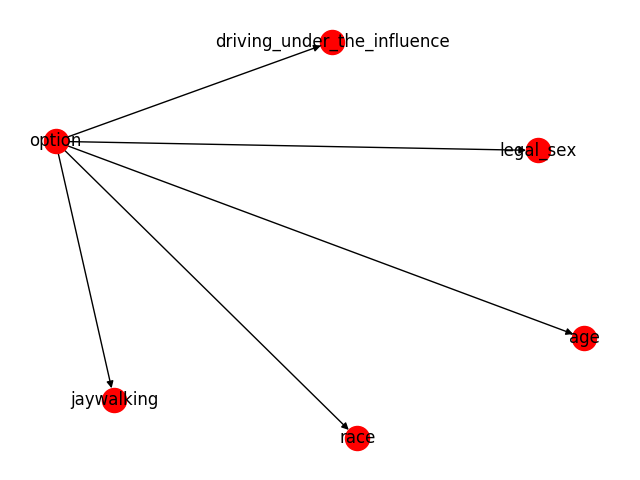
\includegraphics[scale=0.6]{figures/network.png}
    \caption[]{The graphical model.}
    \label{fig:graphical_model_image}
\end{figure}

\begin{figure}[h]
    \centering
    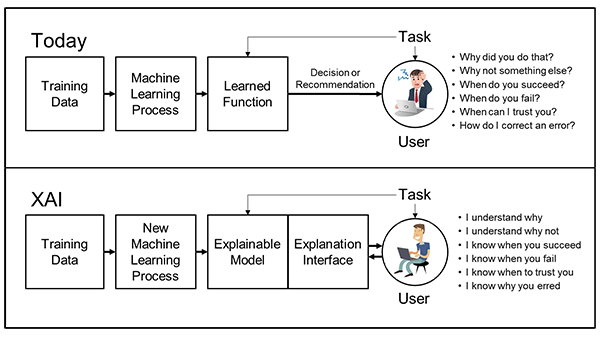
\includegraphics[scale=1.1]{figures/xai-figure2.png}
    \caption[]{DARPA's XAI Concept~\protect\cite[]{gunningXAIProgram}}
    \label{fig:darpa_xai}
\end{figure}

% 
% test 40-60 100-0 0-100
% 

\begin{figure}[h]
    \centering
    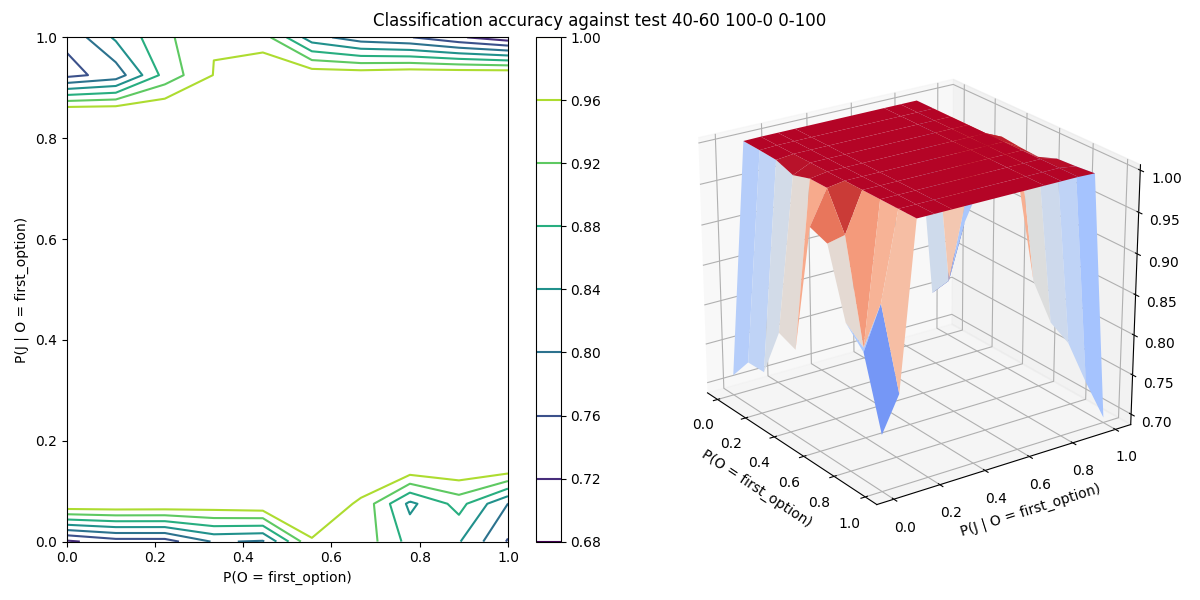
\includegraphics[width=\textwidth]{test_40-60_100-0_0-100_accuracy.png}
    \caption[]{The classification accuracy against \code{test 40-60 100-0 0-100}.}
    \label{fig:test_40-60_100-0_0-100_accuracy_plot}
\end{figure}

\begin{figure}[h]
    \centering
    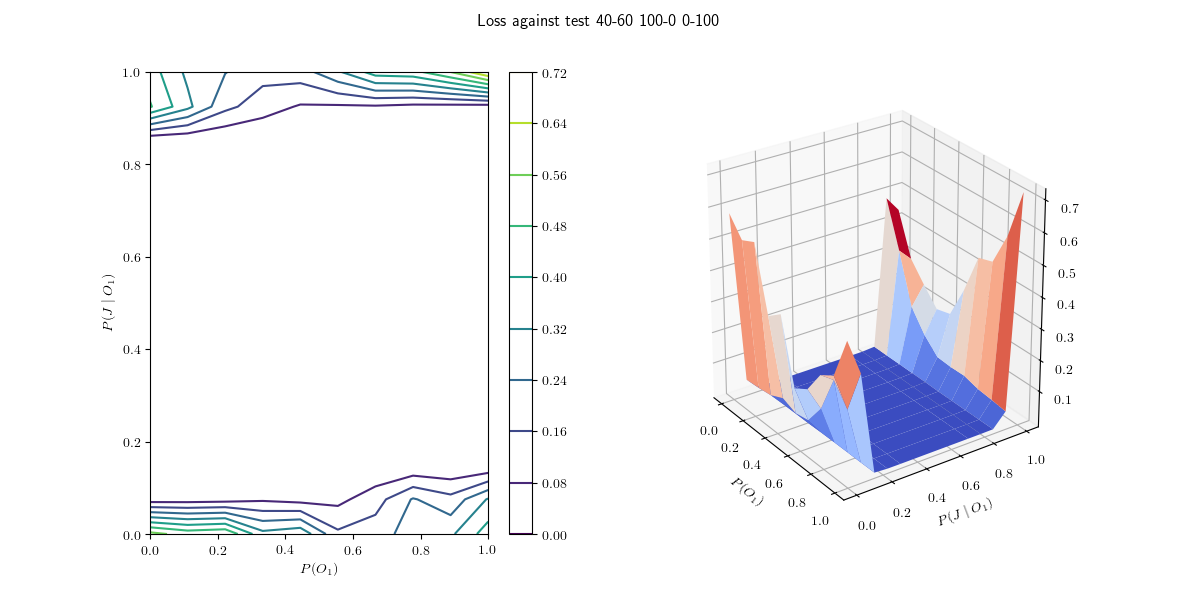
\includegraphics[width=\textwidth]{test_40-60_100-0_0-100_loss.png}
    \caption[]{The loss against \code{test 40-60 100-0 0-100}.}
    \label{fig:test_40-60_100-0_0-100_loss_plot}
\end{figure}

\begin{figure}[h]
    \centering
    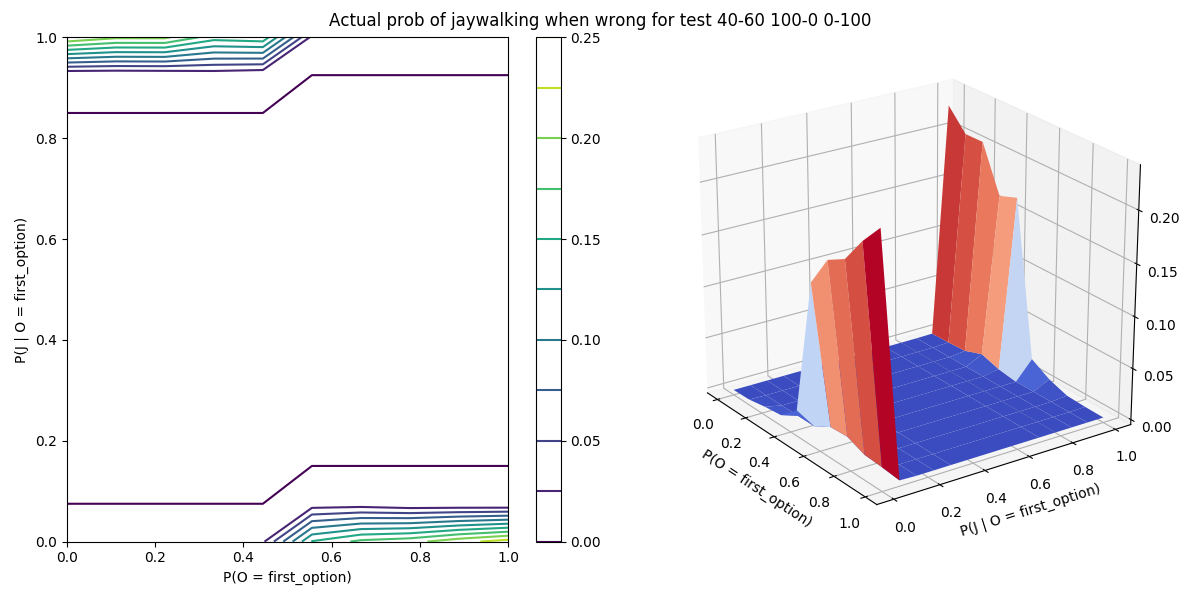
\includegraphics[width=\textwidth]{test_40-60_100-0_0-100_jay_prob.png}
    \caption[]{The actual jaywalking probability when classified incorrectly against \code{test 40-60 100-0 0-100}.}
    \label{fig:test_40-60_100-0_0-100_jay_prob_plot}
\end{figure}

% 
% test 40-60 0-100 100-0
% 

\begin{figure}[h]
    \centering
    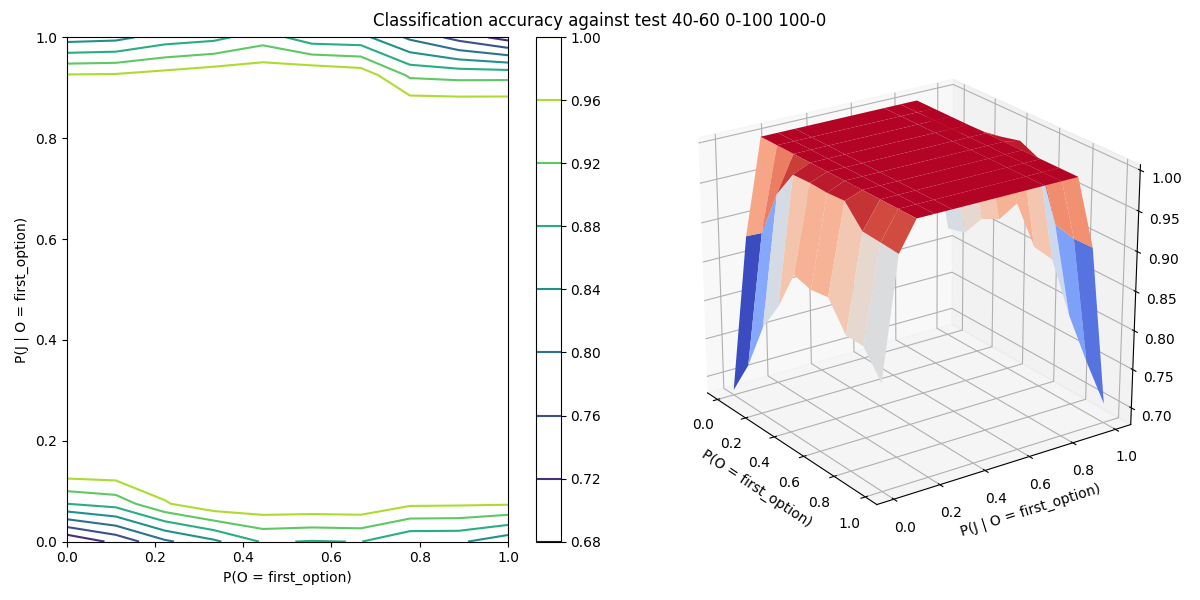
\includegraphics[width=\textwidth]{test_40-60_0-100_100-0_accuracy.png}
    \caption[]{The classification accuracy against \code{test 40-60 0-100 100-0}.}
    \label{fig:test_40-60_0-100_100-0_accuracy_plot}
\end{figure}

\begin{figure}[h]
    \centering
    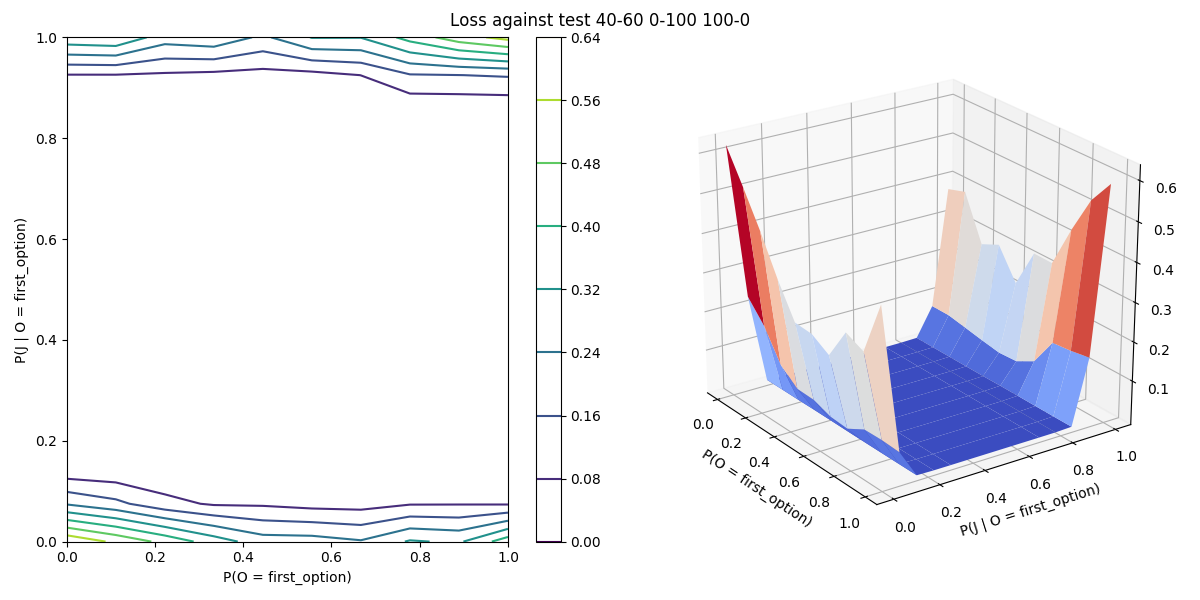
\includegraphics[width=\textwidth]{test_40-60_0-100_100-0_loss.png}
    \caption[]{The loss against \code{test 40-60 0-100 100-0}.}
    \label{fig:test_40-60_0-100_100-0_loss_plot}
\end{figure}

\begin{figure}[h]
    \centering
    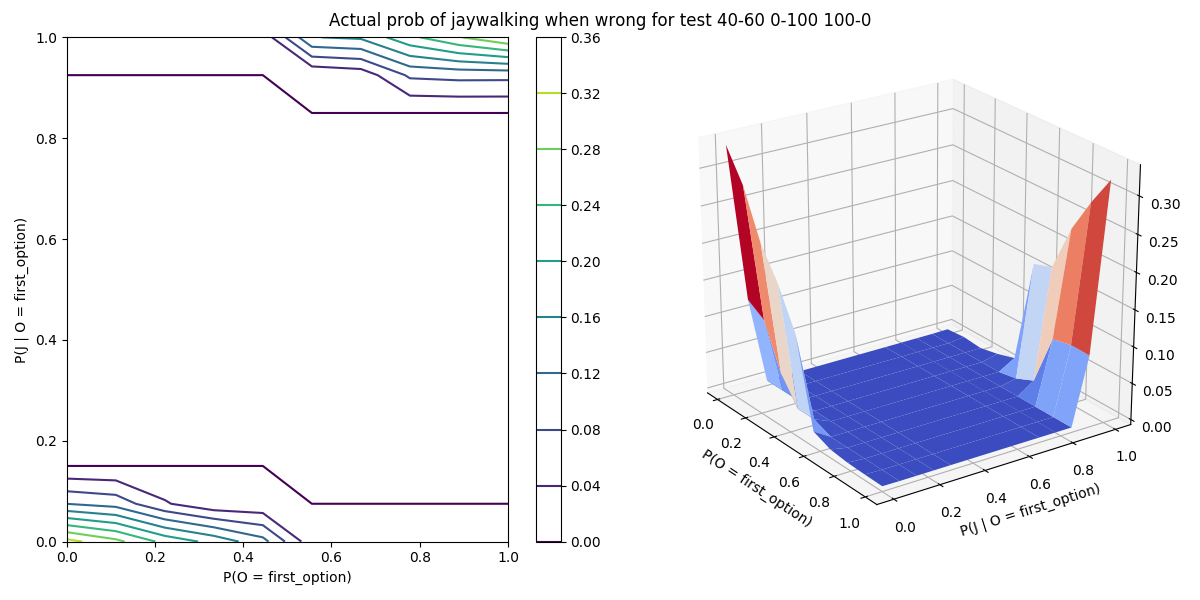
\includegraphics[width=\textwidth]{test_40-60_0-100_100-0_jay_prob.png}
    \caption[]{The actual jaywalking probability when classified incorrectly against \code{test 40-60 0-100 100-0}.}
    \label{fig:test_40-60_0-100_100-0_jay_prob_plot}
\end{figure}

% 
% test 40-60 80-20 20-80
% 

\begin{figure}[h]
    \centering
    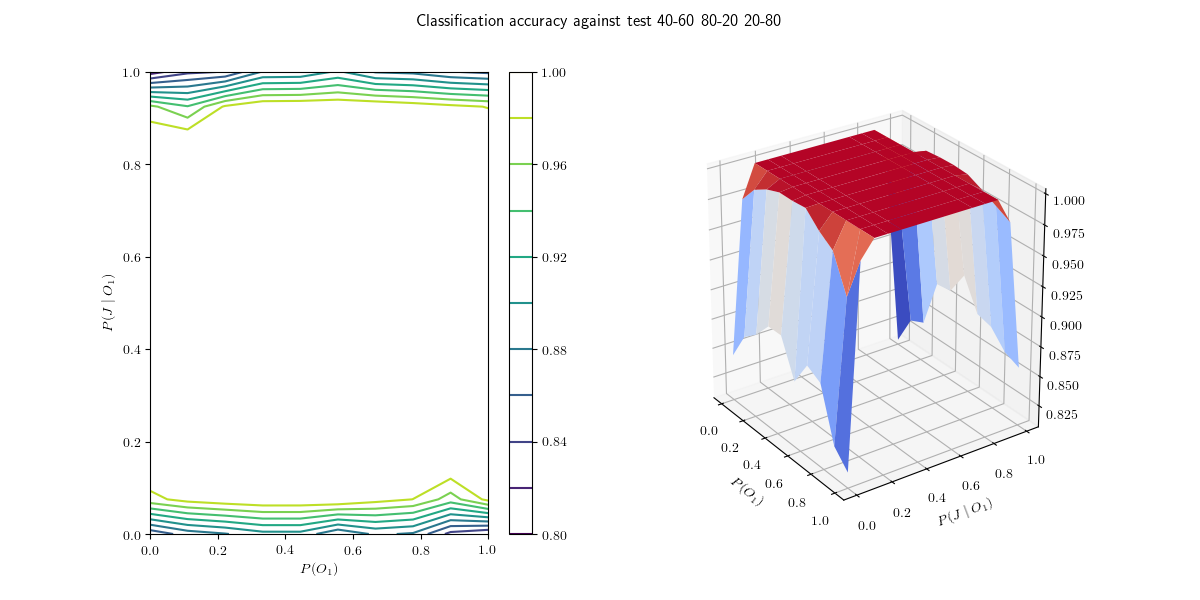
\includegraphics[width=\textwidth]{test_40-60_80-20_20-80_accuracy.png}
    \caption[]{The classification accuracy against \code{test 40-60 80-20 20-80}.}
    \label{fig:test_40-60_80-20_20-80_accuracy_plot}
\end{figure}

\begin{figure}[h]
    \centering
    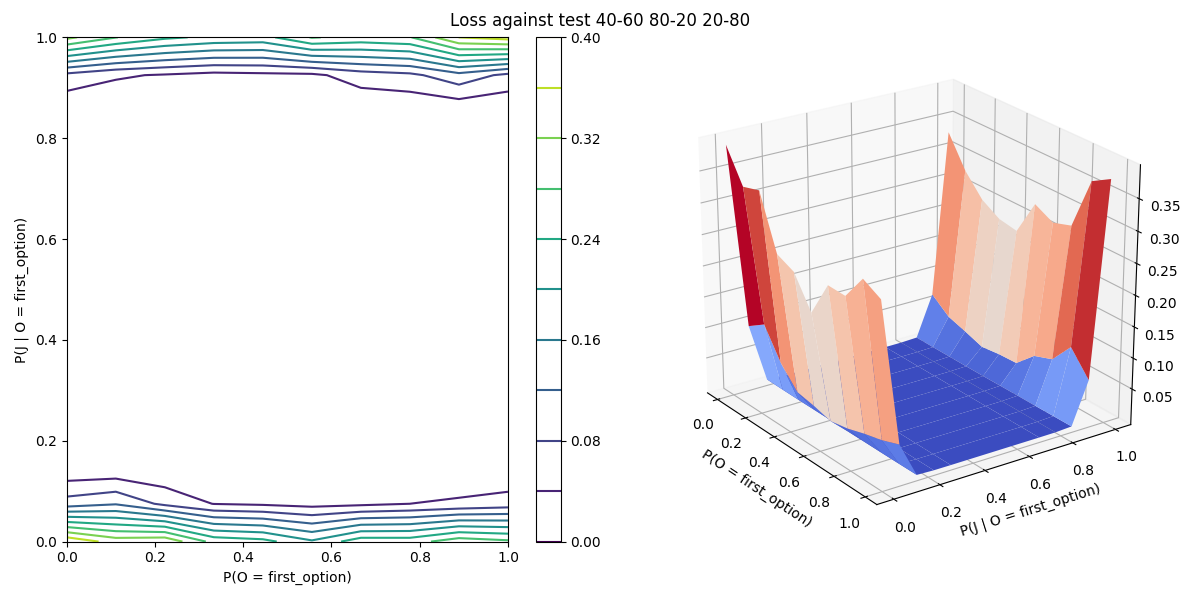
\includegraphics[width=\textwidth]{test_40-60_80-20_20-80_loss.png}
    \caption[]{The loss against \code{test 40-60 80-20 20-80}.}
    \label{fig:test_40-60_80-20_20-80_loss_plot}
\end{figure}

\begin{figure}[h]
    \centering
    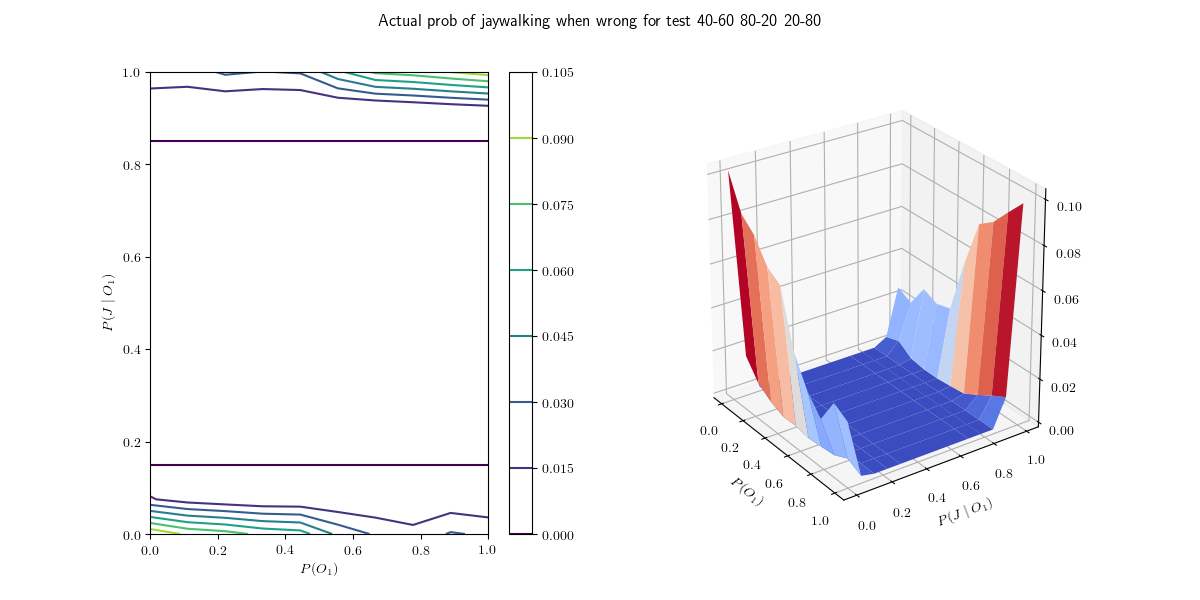
\includegraphics[width=\textwidth]{test_40-60_80-20_20-80_jay_prob.png}
    \caption[]{The actual jaywalking probability when classified incorrectly against \code{test 40-60 80-20 20-80}.}
    \label{fig:test_40-60_80-20_20-80_jay_prob_plot}
\end{figure}

% 
% test 40-60 20-80 80-20
% 

\begin{figure}[h]
    \centering
    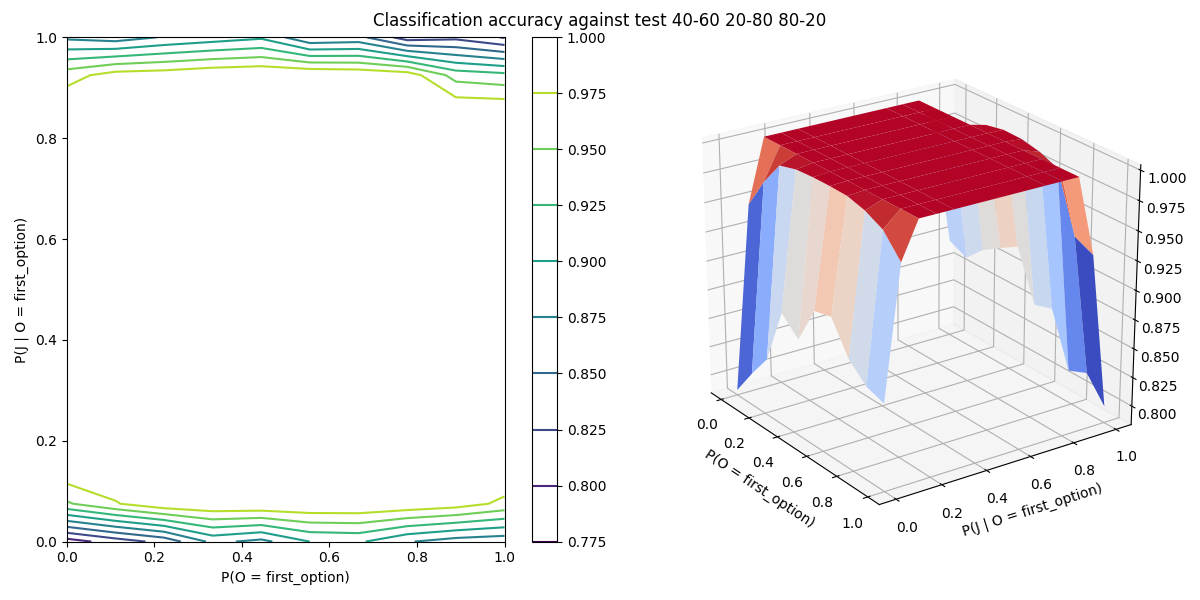
\includegraphics[width=\textwidth]{test_40-60_20-80_80-20_accuracy.png}
    \caption[]{The classification accuracy against \code{test 40-60 20-80 80-20}.}
    \label{fig:test_40-60_20-80_80-20_accuracy_plot}
\end{figure}

\begin{figure}[h]
    \centering
    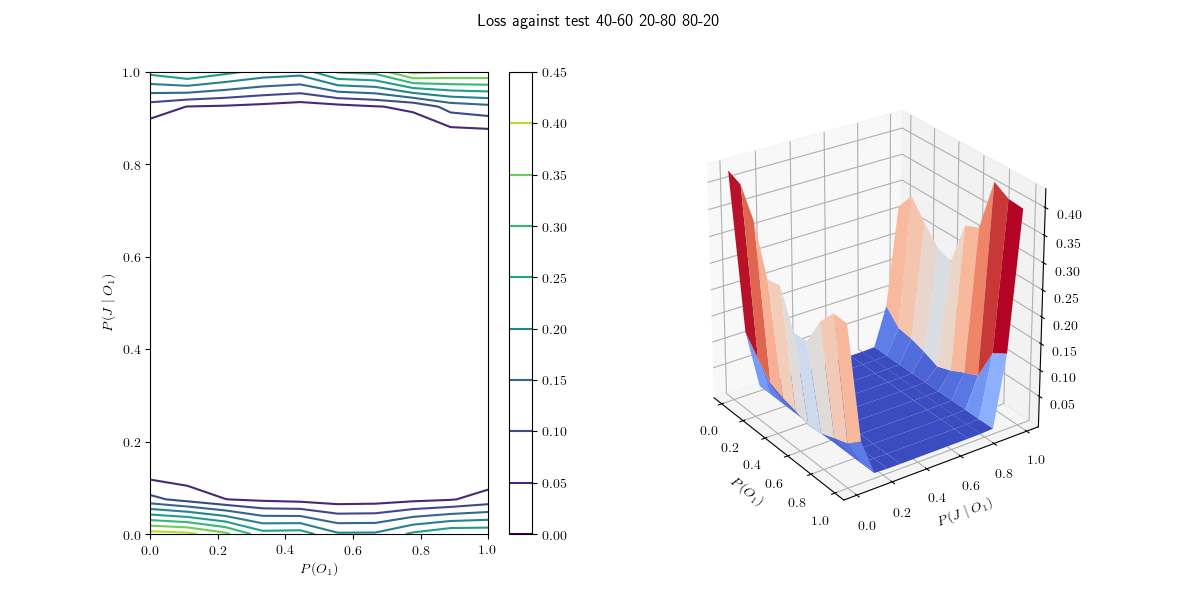
\includegraphics[width=\textwidth]{test_40-60_20-80_80-20_loss.png}
    \caption[]{The loss against \code{test 40-60 20-80 80-20}.}
    \label{fig:test_40-60_20-80_80-20_loss_plot}
\end{figure}

\begin{figure}[h]
    \centering
    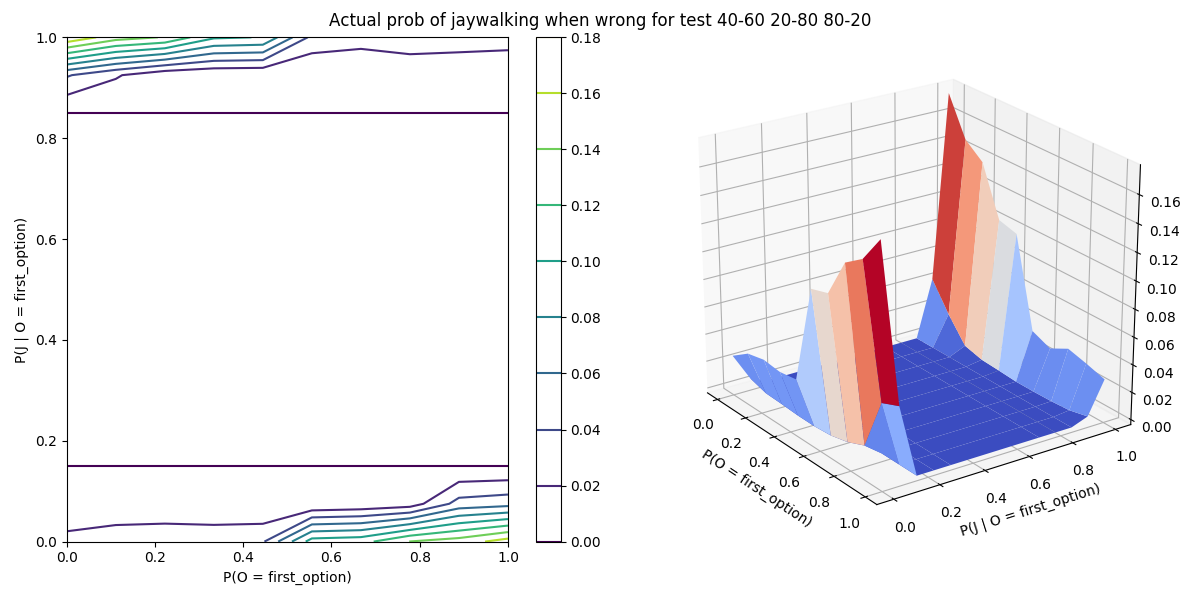
\includegraphics[width=\textwidth]{test_40-60_20-80_80-20_jay_prob.png}
    \caption[]{The actual jaywalking probability when classified incorrectly against \code{test 40-60 20-80 80-20}.}
    \label{fig:test_40-60_20-80_80-20_jay_prob_plot}
\end{figure}

% 
% test 50-50 50-50 50-50
% 

\begin{figure}[h]
    \centering
    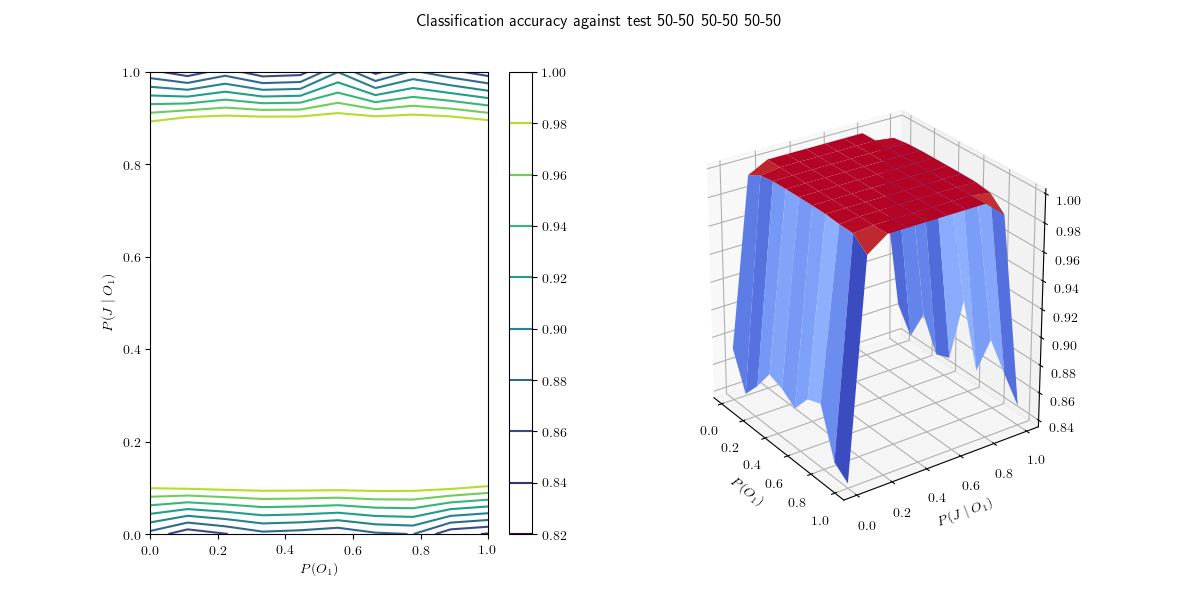
\includegraphics[width=\textwidth]{test_50-50_50-50_50-50_accuracy.png}
    \caption[]{The classification accuracy against \code{test 50-50 50-50 50-50}.}
    \label{fig:test_50-50_50-50_50-50_accuracy_plot}
\end{figure}

\begin{figure}[h]
    \centering
    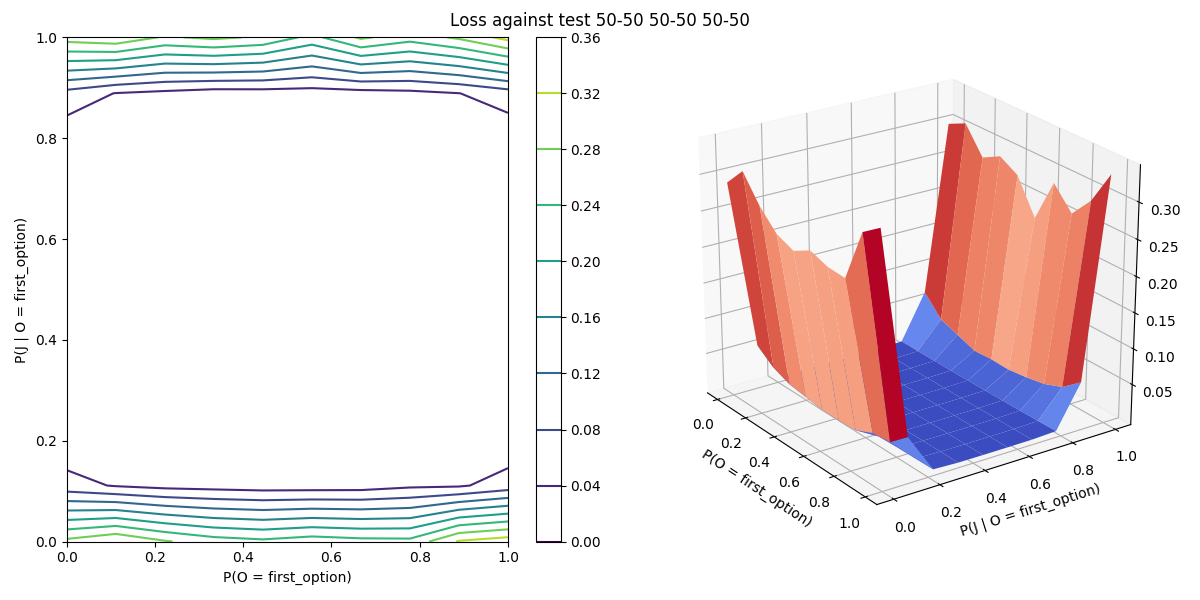
\includegraphics[width=\textwidth]{test_50-50_50-50_50-50_loss.png}
    \caption[]{The loss against \code{test 50-50 50-50 50-50}.}
    \label{fig:test_50-50_50-50_50-50_loss_plot}
\end{figure}

\begin{figure}[h]
    \centering
    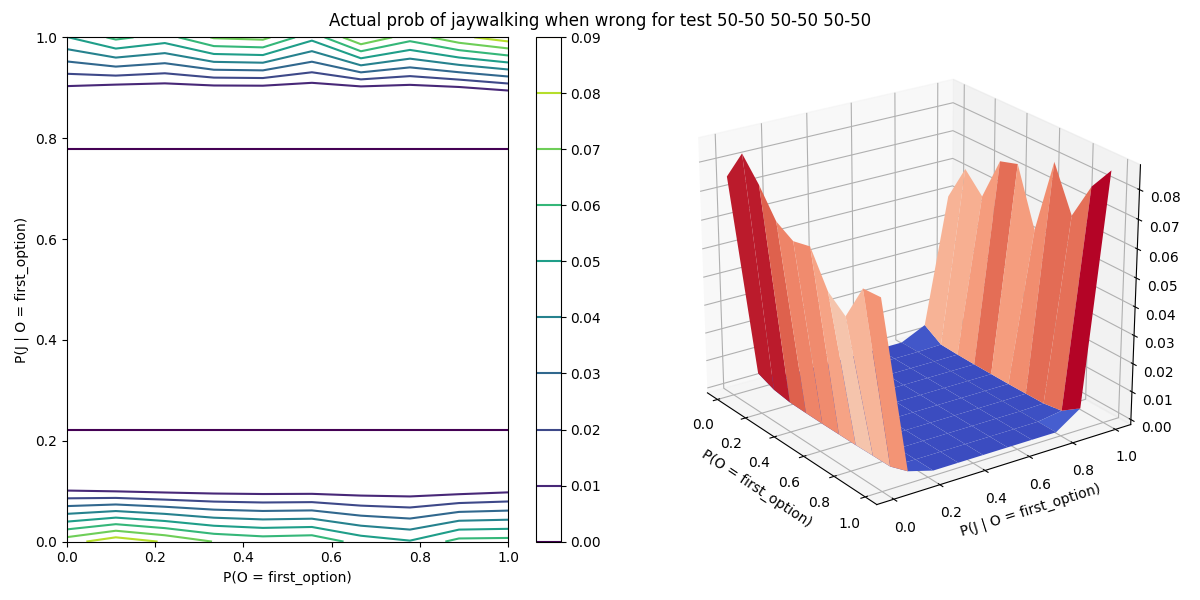
\includegraphics[width=\textwidth]{test_50-50_50-50_50-50_jay_prob.png}
    \caption[]{The actual jaywalking probability when classified incorrectly against \code{test 50-50 50-50 50-50}.}
    \label{fig:test_50-50_50-50_50-50_jay_prob_plot}
\end{figure}

\end{document}
